


\documentclass[letterpaper,11pt]{report}

\usepackage[spanish]{babel} %Lenguaje: Espanol
\usepackage[utf8]{inputenc} %Caracteres: UTF8
\usepackage{graphicx} %Manejo de imágenes

\begin{document}
	\renewcommand{\tablename}{Tabla} %Escribe Tabla en lugar de Cuadro
	\renewcommand{\listtablename}{Índice de tablas} %Escribe Indeice de tablas en lugar de Indice de cuadros
	
	\begin{titlepage}

    \centering %Todo centrado

    %%%%  IMAGEN DE PORTADA Y TÍTULO DE LA IMAGEN   %%%%
    	
\includegraphics[scale=1.2]{imagenes/upiicsa} %Imagen para portada
    	\quad
    	
\includegraphics[scale=0.15]{imagenes/ipn} %Imagen para portada
    	\LARGE{\\ Instituto Polit\'ecnico Nacional} %Título de la imagen
    	\LARGE{\\ Unidad Profesional Interdisciplinaria de Ingeniería y Ciencias Sociales y Administrativas} %Título de la imagen

    	\vspace{1cm} %Espacio vertical

    	%%%%  MATERIA-TRABAJO   %%%%
    	\LARGE {Herramentas Automatizadas\\}
    	\rule{7cm}{3pt} %Línea horizontal
    	\vspace{0.5cm} %Espacio vertical
    	\LARGE \textbf{\\Proyecto Gestión de Alumnos}

    	\vspace{1cm} %Espacio vertical

    	\LARGE {Profesor: Ortega Pacheco José David}

    	\vspace{0.2cm} %Espacio vertical

    	%%%%   ALUMNO Y GRUPO   %%%%
   	Nombre de alumnos:
   	\begin{itemize}
   		\item Castillo López José Roberto
   		\item Jimenez de Anda Raciel
   		\item Martínez Gónzalez Laura
   		\item Pizano Rodríguez Jonathan
   		\item Ortíz Martínez Isaac Bicrí
   	\end{itemize}
    	Secuencia: 2NM50

    	\vspace{0.2cm} %Espacio vertical

    	%%%%   LUGAR Y FECHA   %%%%
		\today

\end{titlepage}
	
	
	    %%%%%%%   INCLUIR ENCABEZADOS EN ÍNDICES Y CAPITULOS   %%%%%%%
	\pagestyle{headings}
	
	%%%%%%%   NUMERACIÓN EN CONTENIDO E ÍNDICE DE TABLAS Y FIGURAS   %%%%%%%
	\pagenumbering{roman} %Números romanos
	%\setcounter{page}{1} %Comienza en I por default, aquí se puedo modificar
	
	%%%%%%   INCLUIR CONTENIDO, ÍNDICE DE FIGURAS Y DE TABLAS   %%%%%%
	\tableofcontents
	\listoffigures
	\listoftables
	
	%%%%%%%   NUMERACIÓN EN CAPÍTULOS   %%%%%%%
	\clearpage %Para iniciar con los arábigos
	\pagenumbering{arabic} %Numeros arábigos
	%\setcounter{page}{1} %Comienza en 1 por default, aquí se puede modificar
	\chapter{Introducción}


\section{Descripción General del Proyecto}
El presente proyecto gestiona los alumnos que se encuentren incritos con un profesor


\section{Propósito}
El propósito del documento es proporcionar la estructura de dicho proyecto para su futuro uso

\section{Alcance del documento}
Dejar en claro los elementos entregados en el documento y hasta que punto se explican o describen. También se llega a describir en algunas ocasiones los elementos que quedan fuera del alcance en el documento, y se dan las razones del por qué, si es que aplica.

\section{Contenido}
Descripción de cada una de las secciones siguientes en el documento

	\chapter{Vista de Escenarios}

	\section{Entregables}

Listado de las historias de usuario que se entregan en el documento, las cuales se detallan a continuación. Se muestre el identificador de cada historia de usuario, el nombre de la historia de usuario, el identificador de la minuta de reunión donde fue aceptada la historia de usuario, así como el nombre del rol o roles involurados participantes en la historia de usuario, así como el nombre de las personas que ocupan los roles.

	\section{Diagrama de casos de uso}
	\begin{figure}[h]
			\centering
			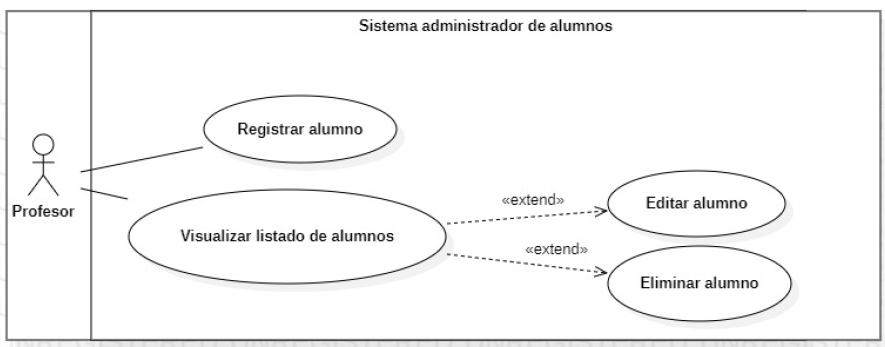
\includegraphics[scale=0.5]{./arquitectura/imagenes/CU1.png}
			\caption{Diagrama de Caso de Uso}
	\end{figure}

	\chapter{Requerimientos}

\section{Requerimientos funcionales}


A continuación, se presenta la lista correspondiente a los requerimientos funcionales del sistema. Asignándole a cada requerimiento un identificador, un nombre y una breve descripción.














\section{Requerimientos no funcionales}

A continuación, se presenta la lista correspondiente a los requerimientos no funcionales del sistema. Dichos requerimietnos se encuentran seccionados en 
\begin{enumerate}
	\item Restricciones de construcción
	\item Identidad gráfica
	\item Propiedades
\end{enumerate} 
Asignándole a cada requerimiento un identificador, un nombre y una breve descripción.\\

\subsection{Restricciones de construcción}

\textbf{RNF1 \hspace{2cm}Sistema operativo Windows 10}\\
Las PC con Windows 10 son rápidas y duraderas, tienen una autonomía increíble y ofrecen un fantástico diseño a un precio  atractivo.  Una nueva PC con Windows 10 es rápida, segura y fiable: todo lo que se necesita para afrontar los desafíos, el caos, las sorpresas y la diversión.\\Windows 10 ofrece antivirus, firewall, antiransomware y protección para Internet, todo ello integrado y sin costo adicional. Además, puedes iniciar sesión de forma rápida y segura mediante el reconocimiento facial o la huella dactilar

\textbf{RNF2 \hspace{2cm}Lenguaje de Programación Java}\\
Java (versión 1.8.0-181 del jdk), es un lenguaje de programación y una plataforma informática. Hay muchas aplicaciones y sitios web que no funcionarán a menos que tenga Java instalado y cada día se crean más. Java es rápido, seguro y fiable. Desde portátiles hasta centros de datos, desde consolas para juegos hasta súper computadoras, desde teléfonos móviles hasta Internet, Java está en todas partes.\\

\textbf{RNF3 \hspace{2cm}IDE Netbeans 8.2}\\
NetBeans IDE es un entorno de desarrollo integrado (IDE) modular y basado en estándares. El proyecto de NetBeans consta de un IDE de código abierto con gran variedad de funciones escrito con el lenguaje de programación Java y una plataforma para aplicaciones de cliente enriquecidas que se puede utilizar como marco genérico para crear cualquier tipo de aplicación
\begin{itemize}
	\item Soporte JavaFX y Java swing
	\item Editor SQL y bases de datos
	\item Soporte multilingüe
	\item Compatibilidad con versiones anteriores \\
\end{itemize}


\textbf{RNF4 \hspace{1cm}Base de datos MySQL Community Edition 8.0.19}\\
MySQL Community Edition es la versión de descarga gratuita de la base de datos de código abierto más popular del mundo. Está disponible bajo la licencia GPL y cuenta con el respaldo de una comunidad enorme y activa de desarrolladores de código abierto.
\begin{itemize}
	\item SQL y NoSQL para desarrollar aplicaciones relacionales y NoSQL
	\item MySQL Document Store que incluye el protocolo X, XDev API y MySQL Shell
	\item Diccionario de datos transaccionales con declaraciones DDL atómicas para mejorar la confiabilidad
	\item Replicación MySQL para mejorar el rendimiento y la escalabilidad de la aplicación
	\item MySQL InnoDB Cluster para ofrecer una solución integrada, nativa y de alta disponibilidad para MySQL
	\item MySQL Router para un enrutamiento transparente entre su aplicación y cualquier servidor MySQL de fondo
	\item Particionamiento MySQL para mejorar el rendimiento y la gestión de grandes aplicaciones de bases de datos
	\item Procedimientos almacenados para mejorar la productividad del desarrollador
	\item Desencadenantes para aplicar reglas comerciales complejas a nivel de base de datos
	\item Vistas para garantizar que la información confidencial no se vea comprometida
	\item Esquema de rendimiento para el monitoreo a nivel de usuario / aplicación del consumo de recursos
	\item Conectores MySQL (ODBC, JDBC, .NET, etc.) para crear aplicaciones en varios idiomas
	\item MySQL Workbench para modelado visual, desarrollo y administración de SQL
	\item Disponible en más de 20 plataformas y sistemas operativos, incluidos Linux, Unix, Mac y Windows.
\end{itemize}

\subsection{Propiedades}

\textbf{RNF5 \hspace{2cm}Eficiencia}\\
Es eficiente, ya que cumple con cada uno de los requisitos establecidos y tiene una óptima productividad en sus componentes. \\

\textbf{RNF6 \hspace{2cm}Complejidad}\\
No cuenta con grado de complejidad el sistema ya que ninguno de sus componentes tiene un diseño o implementación que es difícil de entender y verificar. \\


\textbf{RNF7 \hspace{2cm}Escalabilidad y Heterogeneidad}\\
No cuenta con escalabilidad ya que no tiene la capacidad el sistema de adaptarse a los nuevos requisitos de tamaño y alcance debido su poca complejidad en sus requerimientos y su única función establecida. \\
Si cuenta con la heterogeneidad ya que una de las principales características de Java es que una vez nosotros codificamos un programa este puede ser ejecutado N cantidad de veces en diferentes plataformas. Ya que produce archivos .class y una vez exista este archivo con las instrucciones en ByteCode este puede ser ejecutado en cualquier dispositivo, lo único que podría cambiar entre cada dispositivo es la JVM utilizada, mientras que el archivo se mantiene igual. Todo gracias a la máquina virtual.\\


\textbf{RNF8 \hspace{2cm}Adaptabilidad}\\
El sistema no tiene la capacidad para satisfacer nuevos requisitos y ajustarse a las nuevas condiciones de funcionamiento durante su vida útil ya que solo realiza funciones muy específicas y reducidas, agregar nuevos requisitos generaría un cambio total en la base de datos y en la arquitectura del sistema (diseño).\\


\textbf{RNF9 \hspace{2cm}Confiabilidad}\\
Tiene confiabilidad el sistema ya que realiza su funcionalidad prevista bajo los límites de diseño especificados, sin fallas, durante un tiempo dado, ya que el sistema no es complejo y se puede analizar de manera detallada la seguridad y la verificación de fallas del sistema.\\

\subsection{Identidad gráfica}

\textbf{RNF10 \hspace{2cm}Pantallas}\\
Todas las pantallas tienen un fondo de color blanco y una longitud de 1024 pixeles de ancho por 720 pixeles de ancho\\

\textbf{RNF11 \hspace{2cm}Títulos}\\
Los títulos tienen una tipografía Serif, remarcado en negritas con un tamaño de 36 en color negro\\

\textbf{RNF12 \hspace{2cm}Texto}\\
El texto tiene una tipografía Arial, con un tamaño de 24 y en color negro\\

\textbf{RNF13 \hspace{2cm}Botones}\\
Los botones tienen un tamaño de 200 pixeles de ancho por 45 pixeles de largo.
El fondo está dado en los siguientes colores RGB (1,112,250), con un efecto Hover en color RGB (0,160,255).\\
Su tipografía es Arial, remarcado en negritas, de tamaño 24 y en color blanco.\\

\textbf{RNF14 \hspace{2cm}Cajas de texto}\\
Tienen una longitud de 300 pixeles de ancho por 45 pixeles de largo.
El fondo es de color blanco con tipografía Arial, de tamaño 24 en color negro\\

\textbf{RNF15 \hspace{2cm}Pantallas emergentes (mensajes)}\\
Estas pantallas tienen un tamaño de 600 pixeles de ancho por 300 pixeles de largo, con un borde sencillo dado en color RGB (51,51,255). Siguen el mismo patrón anteriormente descrito en cuanto a texto, títulos y botones.\\






\end{document}